\section{Methodology}

This section details the general methodology used in this report for the design of the overall end system. It consists of a number of stages (Figure 3.1), beginning with an initial research stage followed by a review and planning stage. The design phase then follows and a system prototype is then developed according to user specifications. Stage 4-5 involves experimentation and results analysis of the overall design. Finally the last stage (6) consists of a discussion of the conclusions drawn from this report.

\begin{figure}[H]
\centering
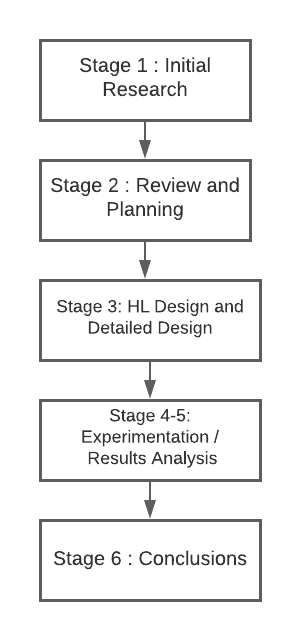
\includegraphics[width=0.28\columnwidth]{Figures/Fig_43.png}
\caption{Methodology stages.}
\label{fig:gantt}
\end{figure}

\subsection{Stage 1 : Initial Research}

The initial research stage aims to develop a theoretical basis for the system design aspect of this report. It consists of a literature review of password security within a broad context. This phase is critical as it lays the foundation for the rest of the report. The approach taken was in exploring the basis of SSO and password managers. Additionally a review of common password attack vectors as well as defenses was explored in order to better understand the potential weak points of the design. Finally a review of some common encryption standards was conducted. This was also an important aspect of the literature review as encryption plays a key role in the secure storage of user credentials.

\subsection{Stage 2 : Review and Planning}

Following the research phase a basic framework for developing the rest of the project was created. This involved developing a Gantt chart with the various phases of the project that required completion. The practical work was divided into both a software and hardware design component.

\subsection{Stage 3 : Design}
Stage 3 includes the synthesis of user requirements to produce a working system prototype. Design of the overall prototype is through an initial high level design phase to establish key system requirements and this is then followed by a detailed design phase where the individual software subsystems of the overall system are implemented in code. Additionally hardware schematics for various system circuitry are also designed. 

\subsection{Stage 4 : Experimentation}

Stage 4 consists of a range of experiments to identify the strength and security of the overall design. Various attack vectors are utilized in an attempt to compromise credential security. The attack vectors identified in the literature review will also be used to develop the required experimentation.

\textbf{Experiment 1 - Malware and Serial tap}

Here a malicious modification to the browser extension (UI element) is made in order to try and capture sensitive data including login credentials. This involves writing JavaScript malware that attempts to make a connection to a command and control server within the extension over a WebSocket connection. Extraction of plain-text credentials through tapping of a serial connection is also attempted using a USB to serial converter. This experiment is aimed at compromising the confidentiality of information.

\textbf{Experiment 2 - Denial of Service}
Various exploitation techniques are tested in an attempt to deny legitimate users access to the services exposed through the end system. This experiment is aimed at disrupting communication between the host device and client software. Denial of service attacks are aimed at disrupting the availability of data.

\textbf{Experiment 3 - Code Injection}
Two types of data exist, namely data in motion which is usually facilitated through a communication protocol between a host and a client and data at rest, which is usually stored on a file system. The data in motion of the overall system consists of the key modulus and plain-text password traversing the software client from the browser. This middle-man client is vulnerable to a range of exploits including function detouring to capture sensitive information. The objective of this experiment is to modify a program such that credential data is leaked and is aimed at compromising data integrity.

\subsection{Stage 5 : Results Analysis}
The results analysis stage (stage 5) then follows the experimentation phase (stage 4). Here data collected from various experiments will be analyzed to determine both strengths and weak points in the design. The data analysis stage therefore plays a key role in making system modifications. The data analysis methodology utilized will mostly involve a qualitative analysis of experimental data against design goals.

\subsection{Stage 6 : Discussion and Conclusions}
The last stage of the methodology involves drawing conclusions and determining if user requirements as well as ATP procedures were met. System performance metrics will also be analyzed. At this point the design should be resilient and key network security objectives should have been met. Potential future work on this topic will also be discussed.


